\chapter{Funciones económicas fundamentales}
\label{cap:funciones}

\section{La idea de función como relación de dependencia}

Casi todo en economía es una \textbf{relación entre dos magnitudes}: la cantidad demandada depende del precio, el costo depende de cuánto producimos, el ingreso depende de cuánto vendemos. La herramienta matemática para capturar «$y$ depende de $x$» es la \emph{función}. Escribir $y = f(x)$ es declarar que, fijado un valor de $x$, queda determinado un valor de $y$.

En este capítulo presentamos las cuatro familias de funciones que vertebran todo el análisis microeconómico de la gestión: \textbf{demanda}, \textbf{oferta}, \textbf{costos} e \textbf{ingreso}, y cómo de ellas surge el \textbf{beneficio}. Seguimos la presentación estándar de \cite{varian} y \cite{pindyck}, simplificada para un primer contacto.

\section{La función de demanda}

\begin{definicion}[Función de demanda]
La \emph{función de demanda} $Q_d = D(p)$ indica la cantidad de un bien que los consumidores están dispuestos a comprar para cada precio $p$, manteniendo todo lo demás constante (\emph{ceteris paribus}).
\end{definicion}

La \textbf{ley de la demanda} establece que, en general, a mayor precio menor cantidad demandada: la función es \emph{decreciente}. Una forma lineal habitual es
\begin{equation}
Q_d = a - b\,p, \qquad a>0,\ b>0,
\label{eq:demanda}
\end{equation}
donde $a$ representa la cantidad que se compraría a precio cero (el «tamaño» potencial del mercado) y $b$ mide cuánto cae la cantidad por cada peso de aumento del precio (la \emph{sensibilidad} al precio).

\subsection*{La demanda inversa}

En muchos problemas de gestión conviene «dar vuelta» la relación y preguntar: \emph{¿a qué precio puedo vender una cantidad $Q$?} Despejando $p$ de \eqref{eq:demanda} obtenemos la \textbf{función de demanda inversa}:
\begin{equation}
p = \frac{a}{b} - \frac{1}{b}\,Q.
\label{eq:demanda_inversa}
\end{equation}
Esta forma es la que usaremos al calcular ingresos y excedentes, porque expresa el precio —lo que entra a la caja por unidad— en función de la cantidad vendida. La distinción entre demanda y demanda inversa, que parece un mero despeje algebraico, es conceptualmente importante y fue uno de los temas que el curso destacó.

\begin{figure}[htbp]
\centering
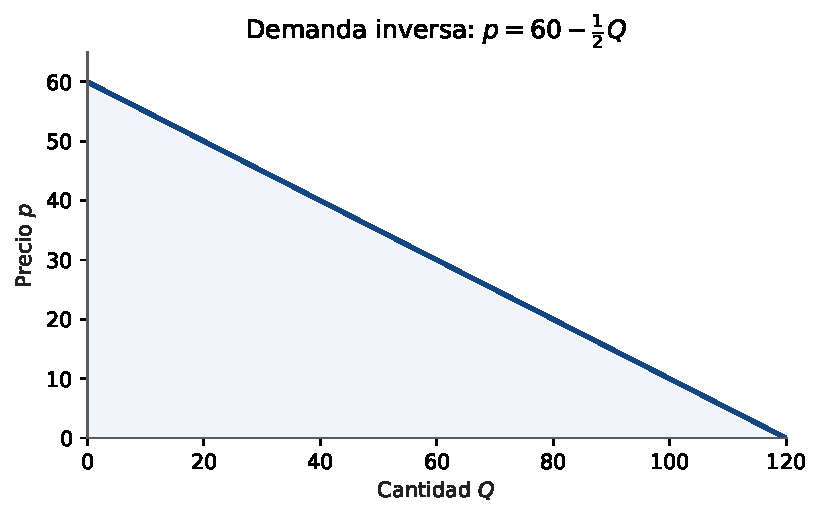
\includegraphics[width=0.72\linewidth]{figuras/demanda_inversa}
\caption{La demanda inversa expresa el precio máximo que el mercado paga por cada cantidad. El área bajo la curva representa la disposición total a pagar.}
\label{fig:demanda_inversa}
\end{figure}

\section{La función de oferta}

\begin{definicion}[Función de oferta]
La \emph{función de oferta} $Q_s = S(p)$ indica la cantidad que los productores están dispuestos a vender para cada precio $p$.
\end{definicion}

A diferencia de la demanda, la oferta suele ser \emph{creciente} en el precio: cuanto más alto el precio, más rentable producir y más unidades se ofrecen. Una forma lineal típica es
\begin{equation}
Q_s = c + d\,p, \qquad d>0.
\label{eq:oferta}
\end{equation}
El parámetro $c$ puede ser negativo: representa que por debajo de cierto precio mínimo no hay oferta (a nadie le conviene producir a pérdida).

\section{Costos: la estructura productiva}

Del lado de la empresa, la magnitud central es el \textbf{costo} de producir una cantidad $q$. Distinguimos:

\begin{itemize}
  \item \textbf{Costo fijo} ($CF$): no depende de la cantidad producida (alquiler, seguros, una máquina). Existe aunque $q=0$.
  \item \textbf{Costo variable} ($CV(q)$): crece con la producción (materia prima, energía, horas de trabajo).
  \item \textbf{Costo total}: $\;C(q) = CF + CV(q)$.
\end{itemize}

A partir del costo total se definen dos costos derivados de enorme importancia para la gestión:
\begin{align}
\text{Costo medio:}\quad & \cme(q) = \frac{C(q)}{q}, \label{eq:cme}\\[4pt]
\text{Costo marginal:}\quad & \cmg(q) = \frac{\dd C}{\dd q}. \label{eq:cmg}
\end{align}
El \textbf{costo medio} responde «¿cuánto me cuesta, en promedio, cada unidad?»; el \textbf{costo marginal} responde «¿cuánto me cuesta producir \emph{una unidad más}?». Volveremos sobre el costo marginal en el Capítulo~\ref{cap:marginal}, porque es una derivada y concentra buena parte de la lógica de las decisiones de producción \cite{nicholson}.

\section{Ingreso y beneficio}

\begin{definicion}[Ingreso total]
El \emph{ingreso total} es lo que la empresa factura: precio por cantidad,
\[
I(q) = p \cdot q.
\]
\end{definicion}

Si la empresa es precio-aceptante (vende a un precio $p$ fijo de mercado), el ingreso es una recta $I(q)=p\,q$. Pero si la empresa tiene poder de mercado y enfrenta la demanda inversa \eqref{eq:demanda_inversa}, el precio baja a medida que quiere vender más, y el ingreso se vuelve \emph{no lineal}:
\begin{equation}
I(q) = p(q)\cdot q = \left(\frac{a}{b} - \frac{1}{b}q\right) q .
\label{eq:ingreso}
\end{equation}

Finalmente, el objetivo habitual de la empresa:
\begin{equation}
\boxed{\;\Pi(q) = I(q) - C(q)\;}
\label{eq:beneficio}
\end{equation}
El \textbf{beneficio} (o utilidad económica) es la diferencia entre lo que entra y lo que sale. Maximizar $\Pi$ es el problema que resolveremos formalmente en el Capítulo~\ref{cap:optimizacion}; por ahora alcanza con tener clara la anatomía: ingreso menos costo.

\begin{ejemplo}[Armando las funciones de un kiosco]
Un kiosco enfrenta una demanda $Q_d = 120 - 2p$ (en unidades por día) y tiene un costo total $C(q) = 50 + 10q$ (en pesos). Entonces:
\begin{itemize}
  \item \emph{Demanda inversa:} despejando $p$, \; $p = 60 - \tfrac{1}{2}q$.
  \item \emph{Ingreso:} \; $I(q) = \left(60 - \tfrac12 q\right)q = 60q - \tfrac12 q^2$.
  \item \emph{Costo medio:} \; $\cme(q) = \dfrac{50+10q}{q} = \dfrac{50}{q} + 10$, que cae a medida que el costo fijo se reparte entre más unidades.
  \item \emph{Costo marginal:} \; $\cmg = 10$ (constante: cada unidad extra cuesta \$10).
  \item \emph{Beneficio:} \; $\Pi(q) = \big(60q - \tfrac12 q^2\big) - \big(50 + 10q\big) = -\tfrac12 q^2 + 50q - 50.$
\end{itemize}
Esta última es una parábola con las ramas hacia abajo: existe una cantidad que la maximiza, lo que anticipa el problema de optimización del Capítulo~\ref{cap:optimizacion}.
\end{ejemplo}

\begin{labbox}
En el laboratorio, estas funciones se representan con \texttt{sympy} (definiendo el símbolo \texttt{q} y escribiendo las expresiones tal cual aparecen acá) y se grafican con \texttt{matplotlib}. La traducción es directa: la ecuación \eqref{eq:beneficio} es, palabra por palabra, la línea \texttt{Pi = I - C} de la notebook. Graficar $\Pi(q)$ permite \emph{ver} dónde está el máximo antes de calcularlo, que es exactamente el puente entre la teoría de este capítulo y la práctica.
\end{labbox}

\section{Síntesis del capítulo}

Vimos que la actividad económica de una organización se describe con un puñado de funciones —demanda, oferta, costos, ingreso— y que de su combinación nace el beneficio. La demanda inversa, el costo marginal y el costo medio son los conceptos que más reaparecerán. En el próximo capítulo ponemos a interactuar demanda y oferta para encontrar el \emph{equilibrio de mercado}.
